\documentclass[a4paper]{article}
\usepackage[T2A]{fontenc}
\usepackage[utf8]{inputenc}
\usepackage[ukrainian]{babel}
\usepackage{tikz}
\usepackage{lastpage} 
\usepackage[left=2.5cm, right=1.5cm, top=1.5cm, bottom=2.5cm]{geometry}
\usepackage{fancyhdr}
% \usepackage{graphicx}

\pagestyle{fancy}
\fancyhf{}
\renewcommand{\headrulewidth}{0pt}
\renewcommand{\footrulewidth}{0pt}
% \pagestyle{empty}

\newcommand{\makrosTitle}[2]{
\thispagestyle{empty}
        \centering
        \textbf{Міністерство освіти і науки України}\\
        \textbf{КИЇВСЬКИЙ ПОЛІТЕХНІЧНИЙ УНІВЕРССИТЕТ}\\[2cm]
        \raggedleft
        Кафедра автоматизації та систем неруйнівного контролю\\
        Група ПМ-11
        \vfill
        \centering
        \textbf{ПРОЕКТУВАННЯ СИСТЕМ АВТОМАТИЗАЦІЇ}\\[1cm]
        \textbf{ЗВІТ З ЛАБОРАТОРНОЇ РОБОТИ №#1}\\[1cm]
        \textbf{#2}
        \vfill
        \begin{flushleft}
            Керівник  \qquad\qquad\quad \hfill\qquad (підпис)\hfill 
            д.т.н., проф. Черепанська І. Ю.\\
            \hfill (дата)\\[2cm]
            Виконавець\hfill (підпис)\hfill Погорєлов Б. Ю.\\
            \hfill (дата)
        \end{flushleft}
        \vfill
        \centering
        2025
}

\newcommand{\makrosFrameBig}[2]{
    \thispagestyle{empty} % Вимикає номер сторінки на першій сторінці
    
    \begin{tikzpicture}[remember picture, overlay]
        \begin{scope}[shift={([xshift = 20 mm, yshift = 10 mm]current page.south west)}]
            \draw[line width=2] (0,0) rectangle (180 mm,277 mm);
        \end{scope}
    \end{tikzpicture}
    
    \begin{tikzpicture}[remember picture, overlay]
        \begin{scope}[shift={([xshift = 20 mm, yshift = 10 mm]current page.south west)}, x=1mm, y=1mm]
            \draw[line width=2] (0,0) rectangle (180,40);
            \draw[line width=2]  (7,40) -- (7, 25);
            \draw[line width=2] (17,40) -- (17, 0);
            \draw[line width=2] (40,40) -- (40, 0);
            \draw[line width=2] (55,40) -- (55, 0);
            \draw[line width=2] (65,40) -- (65, 0);
            \draw[line width=2] (135,25) -- (135,0);
            \draw[line width=2] (140,15) -- (140,20);
            \draw[line width=2] (145,15) -- (145,20);
            \draw[line width=2] (150,25) -- (150,15);
            \draw[line width=2] (165,25) -- (165,15);
        
            \draw (0,35) -- (65, 35);
            \draw[line width=2] (0,30) -- (65, 30);
            \draw[line width=2] (0,25) -- (180, 25);
            \draw (0,20) -- (65, 20);
            \draw (0,15) -- (65, 15);
            \draw (0,10) -- (65, 10);
            \draw (0,5) -- (65, 5);
        
            \draw[line width=2] (135,20) -- (180, 20);
            \draw[line width=2] (135,15) -- (180, 15);
            
            \node at (3.5, 27.5) {Зм.};
            \node at (12, 27.5) {Лист};
            \node at (28.5, 27.5) {№ докум.};
            \node at (47.5, 27.5) {Підпис};
            \node at (60, 27.5) {Дата};
            
            \node at (7, 22.5) {Розроб.};
            \node at (6.5, 17.5) {Перев.};
            \node at (8.5, 7.5) {Н. Контр.};
            \node[align=left] at (5, 2.5) {Затв.};
            
            \node at (142.5, 22.5) {Літ.};
            \node at (157.5, 22.5) {Аркуш};
            \node at (172, 22.5) {Аркушів};
        
            \node[align=left, font=\itshape, anchor=south west, scale=0.9] at (16, 20) {Погорєлов Б.Ю.};
            \node[align=left, font=\itshape, anchor=south west, scale=0.8] at (16, 15) {Черепанська І.Ю.};
            \node[align=left, font=\itshape, anchor=south west, scale=0.8] at (16, 0) {Черепанська І.Ю.};
        
            \node[anchor=center, font=\itshape, scale=1.5] at (122, 32) {#1};
            \node[align=center, font=\itshape, anchor=center] at (100, 12) {#2};
            \node[align=left, font=\itshape, anchor=south west, scale=0.9] at (135, 5) {КПІ ім. І. Сікорського, ПБФ};
            \node[anchor=center, font=\itshape] at (158, 17) {2};
            \node[anchor=center, font=\itshape] at (172, 17) {\pageref{LastPage}};    
        \end{scope} 
    \end{tikzpicture}
}

\newcommand{\makrosFrameSmall}[1]{
    % \thispagestyle{empty} % Вимикає номер сторінки на першій сторінці
    
    \begin{tikzpicture}[remember picture, overlay]
        \begin{scope}[shift={([xshift = 20 mm, yshift = 10 mm]current page.south west)}]
            \draw[line width=2] (0,0) rectangle (180 mm,277 mm);
        \end{scope}
    \end{tikzpicture}
    
    \begin{tikzpicture}[remember picture, overlay]
        \begin{scope}[shift={([xshift = 20 mm, yshift = 10 mm]current page.south west)}, x=1mm, y=1mm]
            \draw[line width=2] (0,0) rectangle (180,15);
            \draw[line width=2] (7,0) -- (7, 15);
            \draw[line width=2] (17,0) rectangle (43,15);
            \draw[line width=2] (55,0) rectangle (64,15);
            \draw[line width=2] (170,0) -- (170, 15);

            \draw[line width=2] (0,5) -- (64, 5);
            \draw               (0,10) -- (64, 10);
            \draw[line width=2] (170,8) -- (180, 8);

            \node[anchor=center, scale=0.8] at (3.5, 2.5) {Змн.};
            \node[anchor=center, scale=0.9] at (12, 2.5) {Арк.};
            \node[anchor=center] at (30, 2.5) {№~докум.};
            \node[anchor=center, scale=0.9] at (49, 2.5) {Підпис};
            \node[anchor=center, scale=0.9] at (59, 2.5) {Дата};
            \node[anchor=center, font=\itshape, scale=1.5] at (115, 7.5) 
                {#1};
            \node[anchor=center] at (175, 12) {Арк.};
            \node[anchor=center] at (175, 4) {\thepage};
            
        \end{scope}
    \end{tikzpicture}
}

% \makrosLab{1}{Шифр}{Назва}
\newcommand{\makrosLab}[3]{ 
    \fancyfoot[C]{\makrosFrameSmall{#2}}
    \makrosTitle{#1}{#3}
    \newpage
    \makrosFrameBig{#2}{#3}
    \raggedright
}


\begin{document}
    \makrosLab{2}{л}{
        Розробка та складання схем \\
        електричних принципових керування \\ 
        промисловими двигунами
    }

    \section*{Тема роботи}
    Розробка та складання схем електричних принципових керування
    промисловими двигунами

    \section*{Мета роботи}
    Вивчити будову та принцип дії промислових двигунів
    різних типів, як складових систем автоматичного
    керування / регулювання / контролю. Навчитися складати схеми електричні
    принципові для керування промисловими двигунами різних типів.

    \section*{Вихідні дані (Варіант 09)}
Для варіанту 9:
\begin{itemize}
    \item Номінальна потужність на валу, \( P_{\text{ном.мех}} = 125 \, \text{кВт} \)
    \item Коефіцієнт потужності, \( \cos \varphi_{\text{ном}} = 0.95 \)
    \item Номінальна швидкість обертання, \( n_{\text{ном}} = 1460 \, \text{об/хв} \)
    \item Коефіцієнт перенавантажної здатності, \( \gamma = 2.3 \)
    \item ККД, \( \eta = 91\% \)
    \item Коефіцієнт кратності пускового струму, \( \alpha = 5.1 \)
    \item Коефіцієнт кратності пускового моменту, \( \beta = 2.35 \)
\end{itemize}

    \newpage 
    
    \section*{Завдання}
Трифазний асинхронний двигун з короткозамкненим ротором має такі параметри:
\begin{enumerate}
    \item напруга живлення: $380/220$ В;
    \item номінальна потужність на валу: $P_{\text{ном.мех}}$;
    \item номінальна швидкість: $n_{\text{ном}}$;
    \item коефіцієнт корисної дії: $\eta$;
    \item коефіцієнт потужності: $\cos \varphi_{\text{ном}}$;
    \item коефіцієнт кратності пускового струму: $\alpha$;
    \item коефіцієнт кратності пускового моменту: $\beta = \frac{M_{\text{пуск}}}{M_{\text{н}}}$;
    \item коефіцієнт перенавантажної здатності: $\gamma = \frac{M_{\text{max}}}{M_{\text{н}}}$.
\end{enumerate}

Двигун увімкнено за схемою "зірка" до мережі з лінійною напругою $U_{\text{лін}} = 380$ В, частотою $f = 50$ Гц.

З врахуванням даних таблиці визначити:
\begin{enumerate}
    \item споживану потужність: активну, реактивну, повну;
    \item споживаний струм;
    \item пусковий струм;
    \item ємність конденсаторів для підвищення $\cos\varphi$ до $0,95$ при вмиканні їх за схемами "зірка" та "трикутник", побудувати векторні діаграми напруги і струмів та трикутник потужностей;
    \item обертаючі моменти двигуна: номінальний, пусковий, критичний;
    \item номінальне і критичне значення ковзання;
    \item обертаючий момент двигуна при значеннях ковзання: $S = 0$; $S_{\text{ном}}$; $0,8S_{\text{кр}}$; $S_{\text{кр}}$; $1,2S_{\text{кр}}$; $0,2$; $0,4$; $0,6$; $0,8$; $1$.
\end{enumerate}
    
    \newpage 
    \section*{Схеми}

\begin{figure}[h]
    \centering
    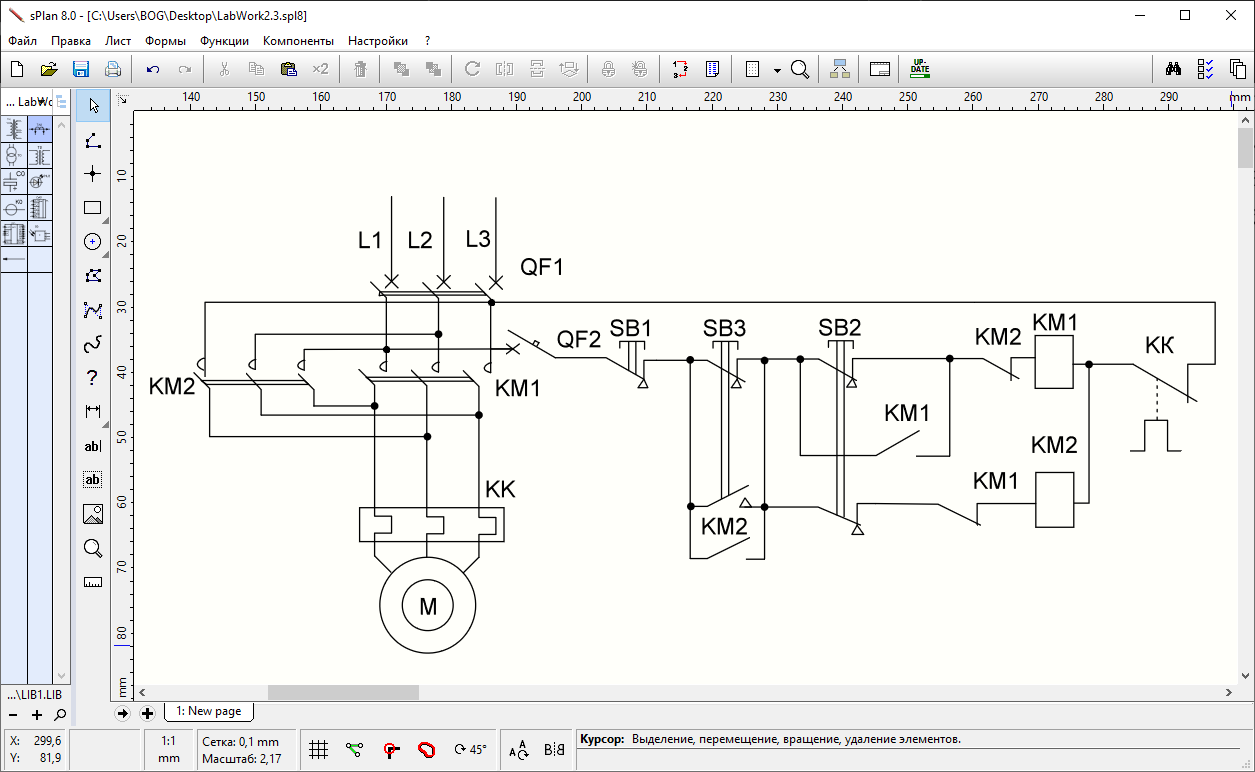
\includegraphics[width=0.8\textwidth]{imgs/LW2.1.png}
    \caption*{Рис. 2.1: Схема електрична принципова реверсивного керування асинхронним електродвигуном}
\end{figure} 

\begin{figure}[h]
    \centering
    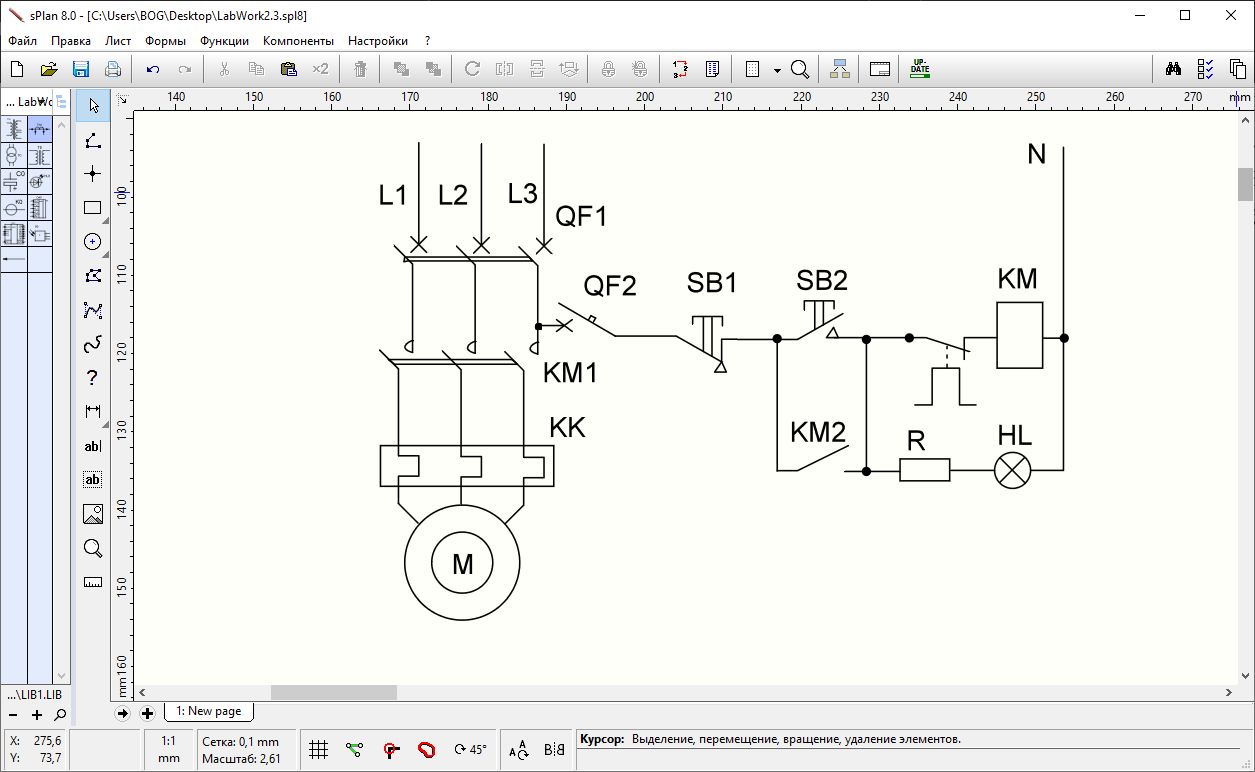
\includegraphics[width=0.85\textwidth]{imgs/LW2.2.png}
    \caption*{Рис. 2.2: Схема електрична принципова нереверсивного керування асинхронним електродвигуном}
\end{figure} 
\newpage
\begin{figure}[h]
    \centering
    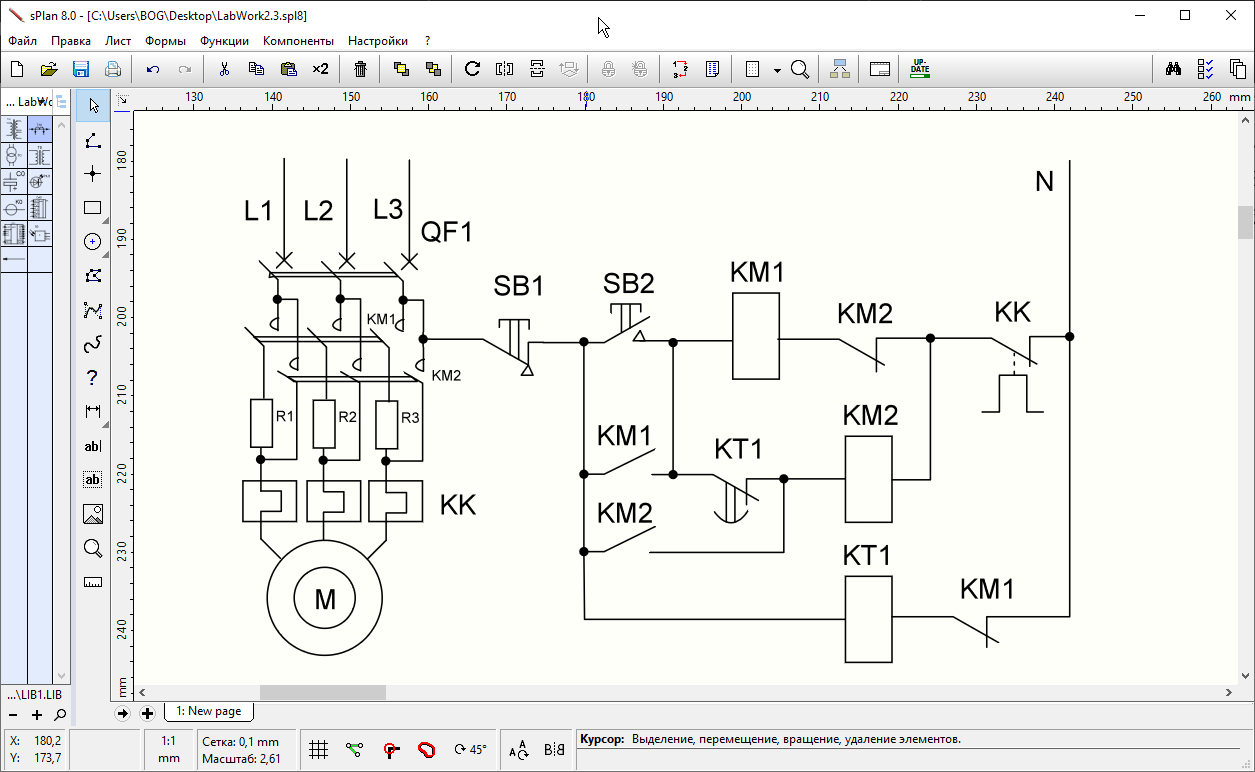
\includegraphics[width=0.65\textwidth]{imgs/LW2.3.png}
    \caption*{Рис. 2.3: Схема електрична принципова керування трифазним асинхронним електродвигуном з короткозамкненим ротором з обмеженням  пускового струму і моменту активними опорами}
\end{figure} 

\begin{figure}[h]
    \centering
    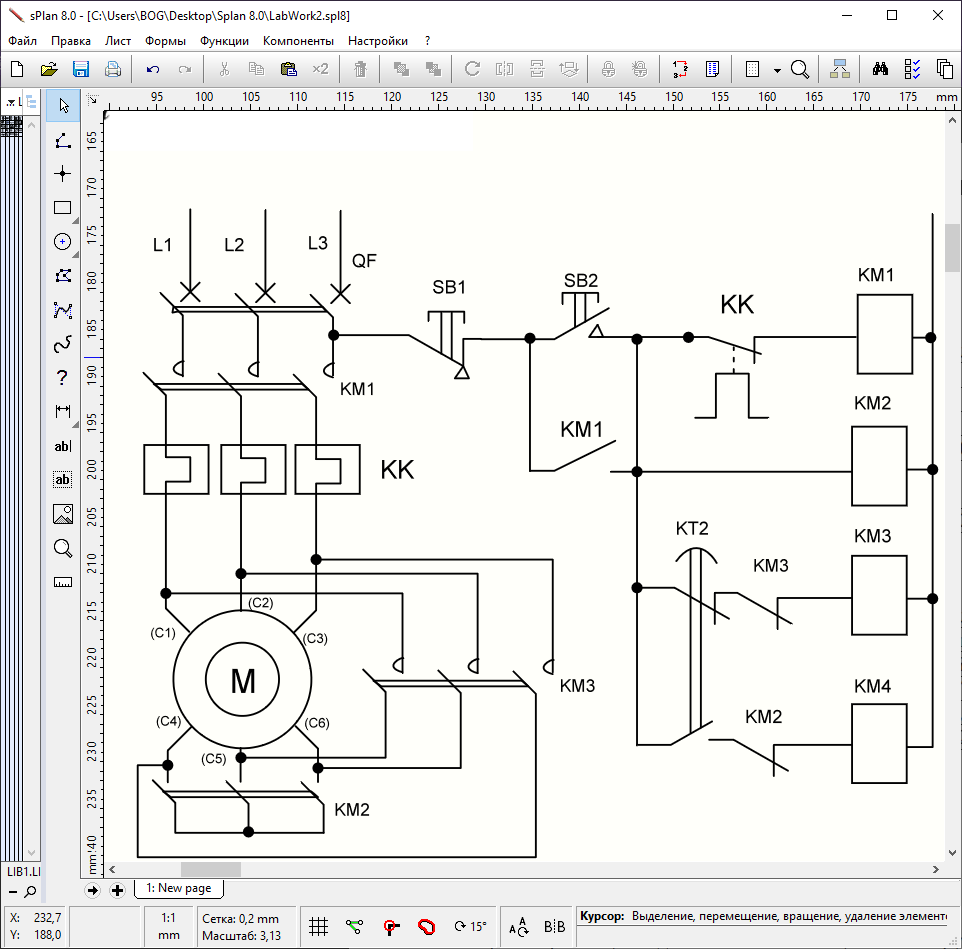
\includegraphics[width=0.55\textwidth]{imgs/LW2.4.png}
    \caption*{Рис. 2.4: Схема електрична принципова керування трифазним асинхронним
електродвигуном з перемиканням обмотки статора iз «зірки» на «трикутник» при пуску}
\end{figure}

\newpage
\begin{figure}[h]
    \centering
    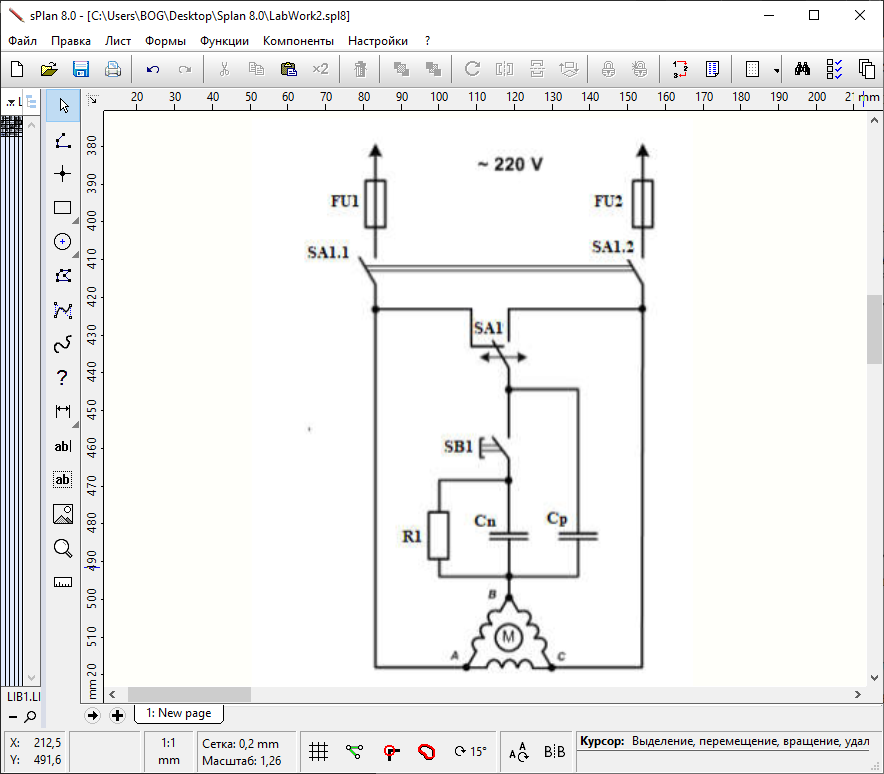
\includegraphics[width=0.7\textwidth]{imgs/LW2.4.2.png}
    \caption*{Рис. 2.5: Схема електрична принципова}
\end{figure}



    \section*{Розрахунки}


\subsection*{1. Споживана потужність}
\textbf{Активна потужність:}
\[
P_{\text{ном.ел}} = \frac{P_{\text{ном.мех}}}{\eta} = \frac{125}{0.91} \approx 137.36 \, \text{кВт}
\]

\textbf{Повна потужність:}
\[
S_{\text{ном}} = \frac{P_{\text{ном.ел}}}{\cos \varphi_{\text{ном}}} = \frac{137.36}{0.95} \approx 144.59 \, \text{кВА}
\]

\textbf{Реактивна потужність:}
\[
Q_{\text{ном}} = \sqrt{S_{\text{ном}}^2 - P_{\text{ном.ел}}^2} = \sqrt{144.59^2 - 137.36^2} \approx 45.16 \, \text{кВАр}
\]

\subsection*{2. Споживаний струм}
\[
I_{л} = \frac{S_{\text{ном}}}{\sqrt{3} \cdot U_{\text{лін}}} = \frac{144.59 \times 10^3}{\sqrt{3} \cdot 380} \approx 219.6 \, \text{А}
\]

\subsection*{3. Пусковий струм}
\[
I_{\text{пуск}} = \alpha \cdot I_{\text{ном}} = 5.1 \times 219.6 \approx 1120 \, \text{А}
\]

\subsection*{4. Ємність конденсаторів для підвищення \( \cos \varphi \) до 0.95}
\textbf{Для схеми "зірка":}
\[
C_Y = \frac{Q_{\text{конд}}}{2 \pi f \cdot 3 U_{ф}^2} = \frac{45.16 \times 10^3}{2 \pi \cdot 50 \cdot 3 \cdot (220)^2} \approx 49.5 \, \mu\text{F}
\]

\textbf{Для схеми "трикутник":}
\[
C_{\Delta} = \frac{Q_{\text{конд}}}{2 \pi f \cdot 3 U_{\text{лін}}^2} = \frac{45.16 \times 10^3}{2 \pi \cdot 50 \cdot 3 \cdot (380)^2} \approx 16.5 \, \mu\text{F}
\]

\subsection*{5. Обертові моменти}
\textbf{Номінальний момент:}
\[
M_{\text{ном}} = \frac{P_{\text{ном.мех}}}{\Omega} = \frac{125 \times 10^3}{2 \pi \cdot \frac{1460}{60}} \approx 818.5 \, \text{Нм}
\]

\textbf{Пусковий момент:}
\[
M_{\text{пуск}} = \beta \cdot M_{\text{ном}} = 2.35 \times 818.5 \approx 1923.5 \, \text{Нм}
\]

\textbf{Критичний момент:}
\[
M_{\text{кр}} = \gamma \cdot M_{\text{ном}} = 2.3 \times 818.5 \approx 1882.6 \, \text{Нм}
\]

\subsection*{6. Ковзання}
\textbf{Номінальне ковзання:}
\[
s_{\text{ном}} = \frac{n_1 - n_{\text{ном}}}{n_1} = \frac{1500 - 1460}{1500} \approx 0.0267
\]

\textbf{Критичне ковзання:}
\[
s_{\text{кр}} = s_{\text{ном}} \cdot \left( \gamma + \sqrt{\gamma^2 - 1} \right) = 0.0267 \cdot \left( 2.3 + \sqrt{2.3^2 - 1} \right) \approx 0.12
\]

\subsection*{7. Потужність втрат}
\textbf{Втрати в обмотках:}
\[
P_{\text{втр}} = P_{\text{ном.ел}} - P_{\text{ном.мех}} = 137.36 - 125 = 12.36 \, \text{кВт}
\]



\section*{Обчислення обертаючого моменту}

Обертаючий момент асинхронного двигуна визначається за формулою:

\begin{equation}
    M = \frac{M_{\text{кр}}}{\frac{S_{\text{кр}}}{S} + \frac{S}{S_{\text{кр}}}}
\end{equation}

де:
\begin{itemize}
    \item $M$ — обертаючий момент двигуна при ковзанні $S$, Н·м;
    \item $M_{\text{кр}}$ — критичний момент (максимальний обертаючий момент), Н·м;
    \item $S$ — значення ковзання;
    \item $S_{\text{кр}}$ — критичне ковзання (значення ковзання, при якому досягається максимальний момент).
\end{itemize}

Ця формула дозволяє обчислити момент для різних значень ковзання:
\begin{itemize}
    \item при $S = 0$ момент теоретично дорівнює нулю;
    \item при $S = S_{\text{кр}}$ двигун розвиває максимальний момент $M_{\text{кр}}$;
    \item при великих значеннях $S$ момент зменшується.
\end{itemize}

\begin{figure}[h]
    \centering
    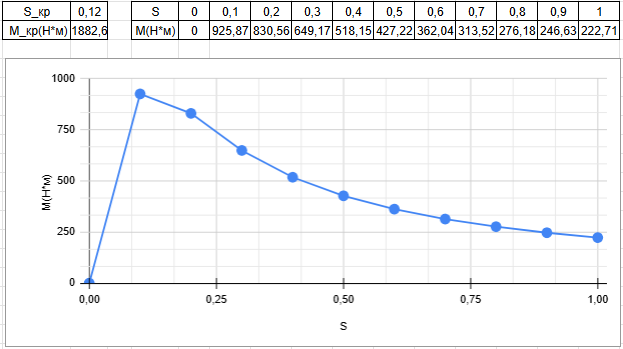
\includegraphics[width=1\textwidth]{imgs/LW2.5.png}
    \caption*{Рис. 2.6: Розрахунок крутного моменту}
\end{figure} 


\section*{Висновки}

Отримані результати дозволяють оцінити параметри роботи трифазного асинхронного двигуна, його енергетичні характеристики та вибір необхідних ємностей для підвищення коефіцієнта потужності.

\section*{Контрольні питання}
\begin{enumerate}
    \item Чому асинхронний двигун так називається? \\
    Асинхронний двигун називається так тому, що частота обертання його ротора не співпадає з частотою обертання магнітного поля статора (яка визначається частотою змінного струму). Різниця між цими частотами називається ковзанням.
    
    \item Чому є небажаною велика сила пускового струму? \\
    Велика сила пускового струму небажана, оскільки вона може призвести до значних механічних та електричних навантажень на двигун і мережу, викликати пошкодження ізоляції проводів, зменшити термін служби обладнання, а також викликати перевантаження трансформаторів і підстанцій.
    
    \item Що використовують для зниження сили пускового струму? \\
    Для зниження сили пускового струму використовують спеціальні пристрої, такі як стартери з обмеженням струму, трансформатори з регульованим напругою або пристрої плавного пуску, що забезпечують поступове збільшення напруги на двигуні.
\end{enumerate}


\end{document}